\chapter{Databases}
First we are going to elaborate on the storage-related architecture of databases in general.
    Then we introduce a popular data model that is employed by many current graph databases~\autocite{GitHubneo4j, ArangoDB, AmazonNeptune, RedisGraph}.
    Finally, at the end of this chapter the implementation of this model in a native graph database called Neo4J is described.
    
\section{Architecture}\label{db-arch}
    The reason why we use databases is twofold:
    First, every computer is equipped with different kinds of memory, which differ in size, capacity, speed and price per byte. 
    This induces the so called memory hierarchy, the principle, that few fast, expensive, low capacity memory is used close to the central processing unit, that gets layerwise augmented with inccreasingly slower, less expensive, higher capacity memory. 
    The last layer, which has the highest capacity, defines the overall capacity, while the smallest one is a crucial factor for performance.
    Thus what is shown as secondary storage in \ref{mem-hier} is orders of magnitude slower in terms of both latency and throughput.
    But it is also able to store orders of magnitude more data. 
    \begin{figure}[htp]
        \begin{center}
        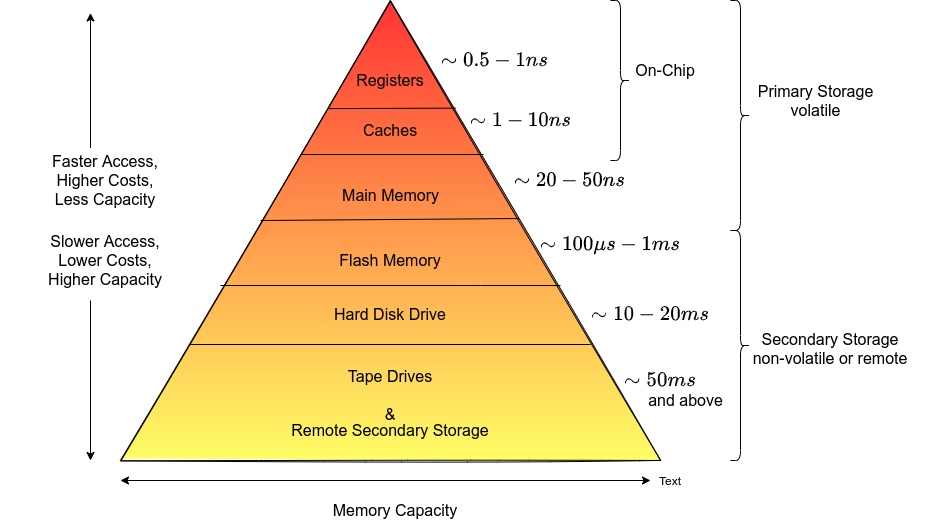
\includegraphics[keepaspectratio,width=0.8\textwidth]{img/04-databases/mem-hierarch.png}
        \end{center}
        \caption{The memory hierarchy used in today's computing systems.} 
        \label{mem-hier}
    \end{figure}
    In order to mitigate the effects of this, the accesses between primary and secondary memory need to be handled very carefully for data intensive --- also called IO bound --- applications.
    Second, the operating system (OS) actually handles the first reason. 
    However application specific payloads enable further optimizations when it comes to how data is stored and accessed.
    Put differently, the operating system is not able to infer certain information, as it does not constrain how data is stored, and as it does not profile in what patterns data is referenced or queried.
    Databases take care of these issues by different mechanisms, which will be lined out from a high level perspective, in order to understand how a database works on its architectural lower levels.
    Put differently, we are not going to discuss query processing, transactions, concurrency related components and recovery facilities.
    Most of the information below is outlined comprehensively in~\autocite{ramakrishnan2000database, silberschatz1997database}
    
    Let us consider the high level architecture of a general database management systems as shown in figure~\ref{dbms_arch} --- with a focus on the storage and access elements.

    \begin{figure}[htp]
    \begin{center}
    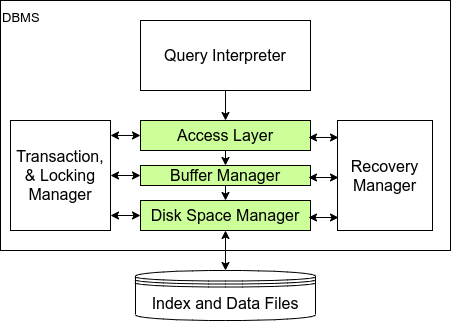
\includegraphics[keepaspectratio,width=.5\textwidth]{img/04-databases/RDBMS.png}
    \end{center}
    \caption{The typical structure of a relational database management system~\autocite{ramakrishnan2000database}.}
    \label{dbms_arch}
    \end{figure}

    The disk space manager, sometimes also called storage manager, handles de-/allocations, reads \& writes and provides the concept of a block: One or many physical disk blocks are grouped to a logical disk block.
    These logical disk blocks are again grouped and brought into main memory (RAM) --- these groups are called a page.
    Optimally both a disk block and a page are of the same size or at least a multiple of each other. 
    Further the database needs to keep track of free blocks in the file: 
    A linked list or a directory must record free blocks and some structure needs to keep track of the free slots either globally or per block. 
    Data locality is a concept that we examine closely in an extra chapter later on.
    To summarize the two most important objectives of a storage manager are to
    \begin{enumerate} 
     \item take care of (de-)allocations of disk space,
     \item abstract storing data on a physical device using the operating system: Files, split into logical disk blocks, accessed using OS facilities, and
     \item provide data structures in order to maintain records within a file, blocks.
    \end{enumerate}
    
    A buffer manager is used to mediate between external storage and main memory. 
    It provides the concept of a page and maintains a designated pre-allocated area of main memory --- called the buffer pool --- to load, cache and evict pages into or from main memory~\autocite{ramakrishnan2000database}.
    A conceptual illustration of this is shown in \ref{buf-man}.
    It's objective is to minimize the number of disk reads to be executed by caching, pre-fetching and the usage of suitable replacement policies. 
    It also needs to take care of allocating a certain fraction of pages to each transaction.

    \begin{figure}[htp]\label{dbms_memory}
        \begin{center}
        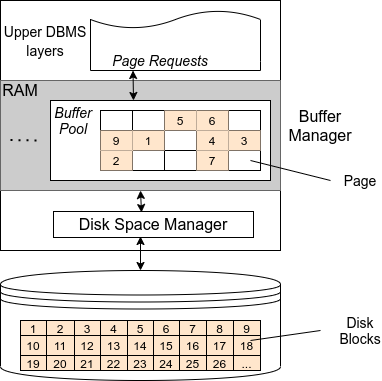
\includegraphics[keepaspectratio,height=0.4\textheight,width=0.5\textwidth]{img/04-databases/RDBMS_memory_view.png}
        \end{center}
        \caption{A visualization of the interaction of a database with memory~\autocite{ramakrishnan2000database}.}
        \label{buf-man}
    \end{figure}

    The final component that is crucial to the storage of data the  of a database management system is the file and record layout, along with possible index structures --- also called the access layer. 
    In order to store data a DBMS may either use one single or multiple files to maintain records. 

    A file consists of a set of blocks split into slots.
    A slot stores one record with each record containing a set of fields.
    Records can be layout in row or column major order.
    That is one can store sequences of tuples or sequences of fields.
    The former is beneficial if a lot of update, insert or delete operations are committed to the database, while the latter optimizes the performance when scans and aggregations are the most typical queries to the system.
    Records may be of fixed or of variable size, depending on the types of their fields. 
    Another option is to store the structure of the records along with pointers to the values of their fields in one files and the actual values in one or multiple separate files. 
    Also distinct types of tables can be stored in different files. 
    For example entities and relations can be stored in different files with references to each other, thus enabling the layout of these two to be specialized to their structure and usage in queries.

    Files may either organize their records in random order (heap file), sorted or using a hash function on one or more fields. 
    All of these approaches have upsides and downsides when it comes to scans, searches, insertions, deletions and updates. 

    To mitigate the effect that result from selecting one file organization or another, one record organization or another, the concept of an index has been introduced. 
    Indexes are auxiliary structures to speed up certain operations or queries that depend on one field. 
    Indexes may be clustered or unclustered. 
    An index over field $F$ is called clustered if the underlying data file is sorted according to the values of $F$. 
    Otherwise the index is called unclustered
    In a similar way indexes can be sparse or dense. 
    A sparse index has less index entries than records, mostly one index entry per block. 
    This can of course only be done for clustered indexes as the sorting of the data file keeps the elements between index keys in order. 
    An index is dense if there is a one to one correspondence between records and index entries. 
    All unclustered indexes are dense indexes.
    There are different variants of storing index entries which have again certain implications on the compactness of the index and the underlying design decisions.
    Finally, there are operators that act upon and use the above structures and mechanisms. 
    Logical operators define an algebraic operation used to process a query.
    Physical operators implement the operation described by logical operators. For each logical operator there may exist multiple different physical implementations using different access methods.

    All these considerations make choosing different file splits, layouts, orderings, addressing schemes, management structures, de-/allocation schemes and indexes a complex set of dependent choices. 
    These depend mainly on the structure of the data to be stored and the queries to be run.
            
\section{Graph Databases}
    Relational databases store data in tables.
    The links considered in this category of DBMS are mostly used to stitch together the fields of a record stored in different tables into one row again, after it has been split to satisfy a certain normal form.
    Of course one may also store tables where one table stores nodes and the other table's fields are node IDs to represent relationships.

    However, in order to traverse the graph, one has either to do a lot of rather expensive look ups or store auxiliary structures to speed up the look up process.
    In particular when using B-trees as index structure, each look up takes $\mathcal{O}(\log(n))$ steps to locate a specific edge.
    Alternatively one could store an additional table that holds incidence lists such that the look up of outgoing or incomming edges is only $\mathcal{O}(\log(n))$ which would speed up breadth first traversals, thus duplicate data.
    But still one has to compute joins in order to continue the traversal in terms of depth.
    Another way to speed things up is to use a hash-based index, but this also has a certain overhead aside from the joins.
    
    In contrast to relational databases, native graph databases use structures specialised for these kinds of queries.
            
    \subsection*{The Property Graph Model}\label{prop-graph-model}
        The property graph model is a widely adopted data model to represent graphs in databases.
        It is not only able to represent the structure of directed or undirected, weighted or unweighted, but also of typed graphs having additional properties.

        A \textbf{Property Graph} is a 9-Tuple $G = (V, E, \lambda, P, T, L, f_P, f_T, f_L)$ with 
        \begin{itemize}
            \item $V$ the set of vertices.
            \item $E$ the set of edges.
            \item $\lambda: (V \times V) \rightarrow E$ a binary relation assigning a pair of nodes to an edge.
            \item $P$ a set of key-value pairs called properties.
            \item $T$ a set of strings used as relationship types.
            \item $L$ a set of strings used as labels.
            \item $f_P: V \cup E \rightarrow 2^P$ a binary relation that assigns a set of properties to a node or relationship.
            \item $f_T: E \rightarrow T$ a binary relation that assigns a type to a relationship.
            \item  $f_L: V \rightarrow 2^L$ a binary relation that assigns a node a set of labels.
        \end{itemize} 
        \smallskip
        The property graph model reflects a directed, node-labeled and relationship-typed multigraph $G$, where each node and relationship can hold a set of properties~\cite{angles2018property, rodriguez2012graph, Rodriguez2010ConstructionsFD}.
        In a graph the edges are normally defined as $E \subseteq (V \times V)$, but in the property graph model edges have sets of properties and a type, which makes them records on their own. 
        An illustration of this model is shown in \ref{propertygraph}.
        
        \begin{figure}[htp]
            \begin{center}
                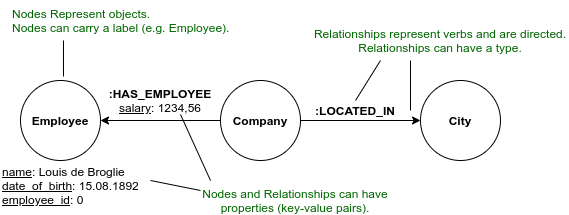
\includegraphics[keepaspectratio,width=0.6\textwidth]{img/04-databases/property_graph_elements.png}
            \end{center}
            \caption{A schematic visualization of the property graph model.} 
            \label{propertygraph}
        \end{figure}

        
        Neo4j is a graph database employing the property graph model~\cite{robinson2015graph}.
        The logical operators of this model are described in~\autocite{Holsch2016Algeb}. 
        The \textit{get\_nodes}-operator returns all nodes of the graph.
        This means that however the nodes are stored, the whole file (portion) needs to be scanned.
        Further the \textit{expand}-operator returns the incident edges of a node depending on the direction.
        Expand only considers a part of the set of all edges, so it does not do full scans but rather smaller reads.
        Finally the \textit{filter}-operand selects certain nodes or relationships based on properties, labels or relationship type.
        
        In the next section \ref{n4j} we are going to discuss how Neo4J implements the property graph model, with our focus on the structure of the graph and the low level storage scheme.

    \subsection*{Example: Neo4J}\label{n4j}
        Neo4J is a native graph database using the property graph model.
        The source code of the community edition is available at GitHub~\autocite{GitHubneo4j}.
        We look at some implementation details of the storage and buffer manager, as well as the record structure.
        We are not going to take properties, relationship types, labels and concepts related to those into account.
        
        \subsubsection*{High-level Architecture}
        \begin{figure}[htp]
            \begin{center}
                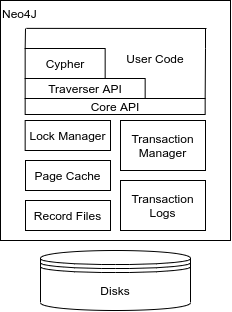
\includegraphics[keepaspectratio,width=0.25\textwidth]{img/04-databases/N4J_HLA_Emil.png}
            \end{center}
            \caption{The high level architecture of Neo4J~\autocite{robinson2015graph}.} 
            \label{N4J_HLA_Emil}
        \end{figure}
        
        To get an overview of the architecture let us consider figure~\ref{N4J_HLA_Emil}.
        This description was outlined by the co-founder of Neo4J Emil Effrem, the chief science officer Jim Webber and Ian Robinson who was an engineer at that time at Neo4J in their book on graph databases~\autocite{robinson2015graph}.
        Here we can see that the architectural schema outlined in \ref{db-arch} and especially \ref{dbms_arch} was not quite applied.
        
        Still the components are very similar:
        The ''Page Cache`` is equivalent to the buffer manager, the record files are what is managed by the disk space manager, mechanisms to deal with free slots~\autocite{neo4jidgenerator} and (de-)allocations~\autocite{neo4jio} are also part of the software stack, as are the record formats~\autocite{neo4jrecordstorage} and indexes, corresponding to the access layer. 
        The corresponding components are just put together in a slightly different manner. 
        
        \begin{figure}[htp]
            \begin{center}
                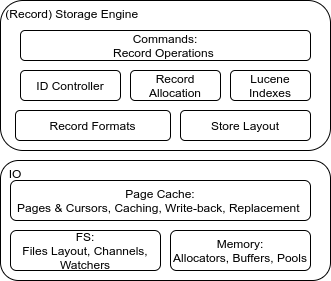
\includegraphics[keepaspectratio,width=0.33\textwidth,height=0.3\textheight]{img/04-databases/N4J_Storage.png}
            \end{center}
            \caption{A visualization of the broad the storage and memory organization of Neo4J.} \label{N4J_Storage}
        \end{figure}
        
        The detailed composition is shown in ~\ref{N4J_Storage}.
        The IO package contains the page cache, which is basically the buffer manager.
        It also contains facilities to create, grow and shrink files using the \mintinline{java}{java.nio} library and wrappers arround platform dependent allocation facilities.
        Thus the (de-)allocation part of the disk space manager resides in the IO package, too.
        The record storage engine defines the record format and the file layout, as well as means to create and maintain indices, thus it is similar to the access layer. 
        It also handles the management of free slots something usually done by the disk space manager.
        To summarize: The buffer manager and the access layer correspond closely to these two packages, while the disk space manager is distributed mainly over these two packages.        

        \subsubsection*{Record and File Structures}
        Neo4J uses several different record types. They can be split broadly in the following categories:
        \begin{itemize}
         \item Variable size records: Strings, Arrays
         \item Fixed size records:
         \begin{itemize}
          \item Graph structure related records: Nodes, relationships, relationship groups
          \item Properties, labels, relationship types
         \end{itemize}
        \end{itemize}
        
        Each record type is stored in an own file per database in the database management system.
        An additional system database keeps track of the existence and metadata of the other ones storing user data.
        This is visualized in~\ref{n4j-disk}.
        \begin{figure}[htp]
            \begin{center}
                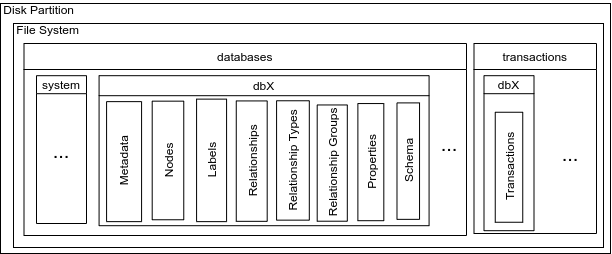
\includegraphics[keepaspectratio,height=0.4\textheight,width=0.7\textwidth]{img/04-databases/N4J_disk_view.png}
            \end{center}
            \caption{A visualization of how the files are arranged of Neo4J.}
            \label{n4j-disk}
        \end{figure}
        
        The records are ordered simply by their insertion order, i.e. the files storing the records are heap files.
        While variable length records store strings and arrays, labels for example store a pointer to the actual string of the label to be fixed size and thus efficiently retreived.
        The same is true for relationship types and property keys and values that are stings or arrays.
        This is done to avoid duplications of strings e.g. of each label.
        As mentioned before for the sake of succintness we are just going to elaborate on the elements that represent the graph structure. 
        Only one thing is to be mentioned: 
        Properties are stored as a linked list for each nodes and relationships.
        
        \subsection*{Nodes}
            \begin{figure}[htp]
                \begin{center}
                    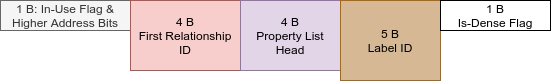
\includegraphics[keepaspectratio,height=0.4\textheight,width=0.7\textwidth]{img/04-databases/node_record.png}
                \end{center}
                \caption{A visualization of the record structure of a node record~\autocite{neo4jNodeRecordFormat}.}
                \label{node-record-format}
            \end{figure}
            The record format of nodes consist of a 15 byte structure.
            The IDs of nodes are stored implicitly as their address.
            If a node has ID 100 we know that its record starts at offset $15 \text{ Bytes} \cdot 100 = 1500$ from the beginning of the file.
            The struct of a record looks like this:
            \begin{enumerate}
                \item Byte 1: One bit for the in-use flag. 
                The additional bits are used to compress the node struct by using the other 7 bits to store the most significant bits of the first relationship ID and the first property ID 
                \item Bytes 2 --- 5: The next 4 Bytes represent the relationship ID of the head in the linked list of relationships of the considered node.
                \item Bytes 6 --- 9: Again 4 bytes encode the property ID 0of the head in the linked list of properties of the node.
                \item Bytes 10 --- 14: This 5 byte section points to the labels of this node.
                \item Byte 15: The last byte stores if the node is dense, i.e.\ has an aweful lot of relationships, such that it needs special treatment in order to remain efficient to traverse over.
                That is a relationships are grouped by type and direction for this node.
            \end{enumerate}
            
            To summarize: The records on disk are stored as in the enumeration above and as shown in \ref{node-record-format}. 
            In the database all IDs get mapped to longs and their respective space is larger than the space representable by 35 bit --- what is perfectly fine.
            
            On disk 4 byte integers are used to store the 32 lowest bits of the respective addresses and the higher bits are stored in the first byte that also carries the in-use bit.
        
        \subsubsection*{Relationships}
            \begin{figure}[htp]
                \begin{center}
                    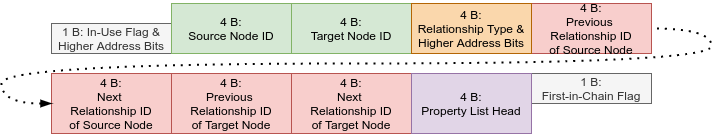
\includegraphics[keepaspectratio,height=0.9\textheight,width=0.9\textwidth]{img/04-databases/relationship_record.png}
                \end{center}
                \caption{A visualization of the record structure of a relationship in Neo4J.}
                \label{rel_record}
            \end{figure}
                
            Relationship records are stored with implicit IDs too. 
            Their fixed size records contain 34 bytes.
            Besides an in-use flag, the source and target node IDs, and the relationship type, the record also contains two doubly linked list: 
            One for the incident edegs of the first node and one for the incident edges of the second node.
            Next a link to the head of the linked list of properties for this relationship is stored.
            Finally, the last byte contains a marker if this relationship is the first element in the incidence list of one of the nodes.
            
            \begin{enumerate}
                \item Byte 1: In-use bit, first node high order bits (3 bits), first property high order bits (4 bits)
                \item Bytes 2 --- 5: first node ID 
                \item Bytes 6 --- 9: second node ID 
                \item Bytes 10 --- 13: relationship type (16 bit), second node high order bits (3 bits), relationship previous and next ID higher bits for first and second node ($4 \cdot 3 = 12$ bits), one unused bit.
                \item Bytes 14 --- 17: previous relationship ID for first node
                \item Bytes 18 --- 21: next relationship ID for first node
                \item Bytes 22 --- 25: previous relationship ID for second node
                \item Bytes 26 --- 29: next relationship ID for second node
                \item Bytes 30 --- 33: link to the first property of the relationship
                \item Bytes 34: A marker if this relation is the first element in the relationship linked list of one of the nodes stored in the lowest two bits of the byte. 
                The other 6 bits are unused.
            \end{enumerate}
            
            \begin{figure}[htp]
                \begin{center}
                    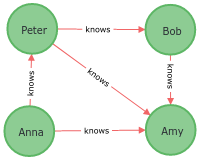
\includegraphics[keepaspectratio,height=0.4\textheight,width=0.3\textwidth]{img/04-databases/graph.png}
                \end{center}
                \caption{An example graph.}
                \label{n4j-ex-gr}
            \end{figure}
            
            The relationship structure is a key element of the layout and reveals the actual data type that the database is using:
            Nodes and relationships are both stored once only (i.e. nothing is duplicated).
            Without taking the fields into account, this is an unordered edge list.
            When taking the linked lists of relationships into account, it turns out that the underlying data structure is that of an indicence list, with a couple of additional properties.
            
            First, as already mentioned, the edges are not physically duplicated but only referenced. 
            The records are fixed sized, so addressing them is done by multiplying the index by the size of an entry, meaning one does not need to store primary keys explicitly and adress translation can be done using a simple multiplication. 
            Theoretically one could align the record size to a power of two to turn the multiplication into a bit shift.
            Next, as doubly linked lists are used, the deletion of an edge is in $\mathcal{O}(1)$ if the ID is known.
            If this was not the case, the incidence list would need to be traversed in order to find the previous element.
            Also, the incidence list is stored in the relationships.
            Thus in order to traverse from one node's incidence list to another, there is no need to load the node record itself.
            It suffices to just dereference the next element in the incidence list stored by the relationships, along with storing the ID of the edge that started the traversal.
            This makes the assumption, that the doubly linked incidence lists is circular, i.e. the head's pervious element is the tail and reciprocally.

            To conclude this example, we briefly visualize the just described storage schema. 
            The high-level graph is shown in \ref{n4j-ex-gr}.
            It contains four nodes and five edges.
            The underlying instantiated data structures are shown in \ref{n4j-ex}.
            The light red arcs represent edges, the light green circles nodes.
            The colored boxes on the edges and nodes represent the data structures.
            The brighter red edges represent the doubly linked incidence lists.
            Notice, that the heads and tails of the doubly linked incidence lists are marked by ''X`` to avoid to draw additional edges.
            The brighter green arrows represent the source and target nodes, as stored by the edges.
            \vfill
            \begin{figure}[htp]
                \begin{center}
                    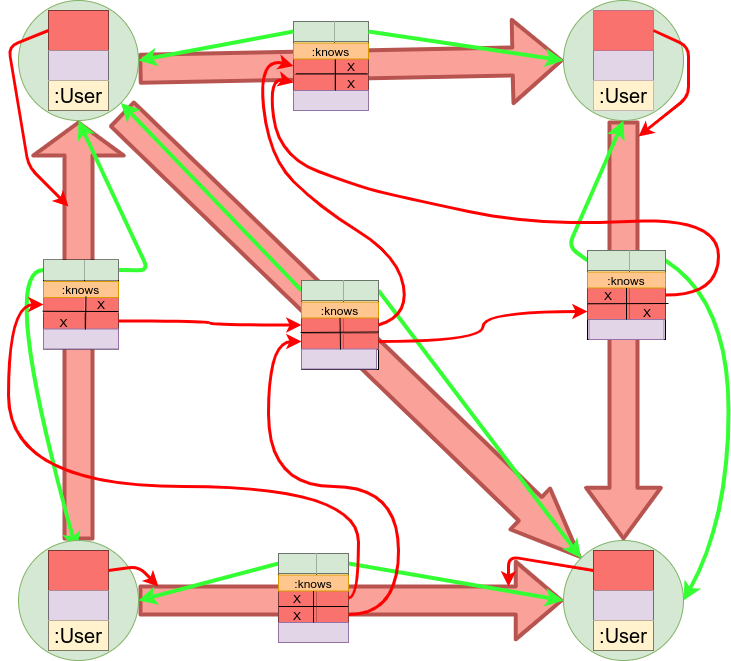
\includegraphics[keepaspectratio,height=\textheight,width=\textwidth]{img/04-databases/example_structs.png}
                \end{center}
                \caption{Visualization of the data structures, as initialized by the example graph shown in \ref{n4j-ex-gr}.}
                \label{n4j-ex}
            \end{figure}
            \vfill
